\documentclass[a4paper,12pt,twoside,openany]{report}
%
% Wzorzec pracy dyplomowej
% J. Starzynski (jstar@iem.pw.edu.pl) na podstawie pracy dyplomowej
% mgr. inż. Błażeja Wincenciaka
% Wersja 0.1 - 8 października 2016
%
\usepackage{listings}
\usepackage{polski}
\usepackage{helvet}
\usepackage{caption}
\usepackage[T1]{fontenc}
\usepackage{anyfontsize}
\usepackage[utf8]{inputenc}
\usepackage[pdftex]{graphicx}
\usepackage{caption}
\usepackage{tabularx}
\usepackage{array}
\usepackage{subfigure}
\usepackage{amsfonts}
\usepackage{algorithmicx}
\usepackage{gnuplottex}
\usepackage{algpseudocode}
\usepackage{algorithm}
\usepackage{verbatim}
\usepackage{indentfirst}
\usepackage[pdftex]{hyperref}
\usepackage{bm}
\usepackage{amsmath}
\usepackage{multicol}

% rozmaite polecenia pomocnicze
% gdzie rysunki?
\graphicspath{ {rys/} }
% oznaczenie rzeczy do zrobienia/poprawienia
\newcommand{\TODO}{\textbf{TODO}}
\newcommand*\NewPage{\newpage\null\thispagestyle{empty}\newpage}



% wyroznienie slow kluczowych
\newcommand{\tech}{\texttt}

% na oprawe (1.0cm - 0.7cm)*2 = 0.6cm
% na oprawe (1.1cm - 0.7cm)*2 = 0.8cm
%  oddsidemargin lewy margines na nieparzystych stronach
% evensidemargin lewy margines na parzystych stronach
\def\oprawa{1.05cm}
\addtolength{\oddsidemargin}{\oprawa}
\addtolength{\evensidemargin}{-\oprawa}

% table span multirows
\usepackage{multirow}
\usepackage{enumitem}    % enumitem.pdf
\setlist{listparindent=\parindent, parsep=\parskip} % potrzebuje enumitem

%%%%%%%%%%%%%%% Dodatkowe Pakiety %%%%%%%%%%%%%%%%%
\usepackage{prmag2017}   % definiuje komendy opieku,nrindeksu, rodzaj pracy, ...
\usepackage{xspace}

%%%%%%%%%%%%%%% Strona Tytułowa %%%%%%%%%%%%%%%%%
% To trzeba wypelnic swoimi danymi
\title{Aplikacja do rozpoznawania emocji w sygnale mowy}

% autor
\author{Wojciech Decker}
\nrindeksu{252545}


\opiekun{dr inż. Andrzej Majkowski}
%\konsultant{prof. Dzielny Konsultant}  % opcjonalnie
\terminwykonania{1 września 2017} % data na oświadczeniu o samodzielności
\rok{2018}


% Podziekowanie - opcjonalne
\podziekowania{\noindent
{\Large Podziękowania}
\bigskip

Dziękujemy bardzo serdecznie wszystkim, a w szczególności Rodzinom i~Unii Europejskiej...

\bigskip

{\raggedleft
Zdolny Student i Pracowity Kolega

}

}

% To sa domyslne wartosci
% - mozna je zmienic, jesli praca jest pisana gdzie indziej niz w ZETiIS
% - mozna je wyrzucic jesli praca jest pisana w ZETiIS
%\miasto{Warszawa}
%\uczelnia{POLITECHNIKA WARSZAWSKA}
%\wydzial{WYDZIAŁ ELEKTRYCZNY}
%\instytut{INSTYTUT ELEKTROTECHNIKI TEORETYCZNEJ\linebreak[1] I~SYSTEMÓW INFORMACYJNO-POMIAROWYCH}
\zaklad{ZAKŁAD SYSTEMÓW INFORMACYJNO POMIAROWYCH}
%\kierunekstudiow{INFORMATYKA}

% domyslnie praca jest inzynierska, ale po odkomentowaniu ponizszej linii zrobi sie magisterska
\pracamagisterska
%%% koniec od P.W

\opinie{%
	\newpage
\begin{center}
 {\large\bf  Opinia} \\
o pracy dyplomowej magisterskiej wykonanej przez dyplomanta\\
{\bf Zdolnego Studenta i Pracowitego Kolegę} \\
 Wydział Elektryczny, kierunek Informatyka,  Politechnika Warszawska\\
Temat pracy\\
\textit{\bf
TYTUŁ PRACY DYPLOMOWEJ
}\\
\end{center}
\medskip
\noindent
Promotor: {\bf dr inż. Miły Opiekun}\\
Ocena pracy dyplomowej: {\bf bardzo dobry}

\medskip

\centerline{\bf Treść opinii}
   Celem pracy dyplomowej panów dolnego Studenta i Pracowitego Kolegi  było
opracowanie systemu pozwalającego symulować  i opartego o oprogramowanie o
otwartych źródłach (ang. Open Source). Jak piszą Dyplomanci, starali się opracować
system, który łatwo będzie dostosować do zmieniających się dynamicznie wymagań,
będzie miał niewielkie wymagania sprzętowe i umożliwiał dalszą łatwą rozbudowę oraz
dostosowanie go do potrzeb.
Przedstawiona do recenzji praca składa się z krótkiego wstępu jasno i
wyczerpująco opisującego oraz uzasadniającego cel pracy, trzech rozdziałów (2-4)
zawierających opis istniejących podobnych
rozwiązań, komponentów rozpatrywanychjako kandydaci do
tworzonego systemu i wreszcie zagadnień wydajności wirtualnych
rozwiązań. Piąty rozdział to opis przygotowanego przez
Dyplomantów środowiska obejmujący opis konfiguracji
środowiska oraz przykładowe ćwiczenia laboratoryjne. Ostatni
rozdział pracy to opis możliwości dalszego
rozwoju projektu. W ramach przygotowania pracy Dyplomanci zebrali i przedstawili w
bardzo przejrzysty sposób duży zasób informacji, co świadczy o dobrej orientacji
w nowoczesnej i ciągle intensywnie rozwijanej tematyce stanowiącej
zakres pracy i o umiejętności przejrzystego przedstawienia tych
wyników. Praca zawiera dwa dodatki, z których pierwszy obejmuje wyniki
eksperymentów i badań nad wydajnością, a drugi to źródła
skryptów budujących środowisko.

 Dyplomanci dość
dobrze zrealizowali postawione przed nimi zadanie,
wykazali się więc umiejętnością zastosowania w praktyce wiedzy
przedstawionej w rozdziałach 2-4.  Uważam, że cele postawione w założeniach pracy zostały pomyślnie
zrealizowane. Proponuję ocenę bardzo dobrą (5).

\vskip 1cm
{
\raggedleft
(data, podpis)\kern1cm

}
	\newpage
	\newpage
\begin{center}
 {\large\bf  Recenzja } \\
pracy dyplomowej magisterskiej wykonanej przez dyplomanta\\
{\bf Zdolnego Studenta i Pracowitego Kolegę} \\
 Wydział Elektryczny, kierunek Informatyka,  Politechnika Warszawska\\
Temat pracy\\
\textit{\bf
TYTUŁ PRACY DYPLOMOWEJ
}\\
\end{center}
\medskip
\noindent
Recenzent: {\bf prof. nzw. dr hab. inż. Jan Surowy}\\
Ocena pracy dyplomowej: {\bf bardzo dobry}
\medskip


\centerline{\bf Treść recenzji}
   Celem pracy dyplomowej panów dolnego Studenta i Pracowitego Kolegi  było
opracowanie systemu pozwalającego symulować  i opartego o oprogramowanie o
otwartych źródłach (ang. Open Source). Jak piszą Dyplomanci, starali się opracować
system, który łatwo będzie dostosować do zmieniających się dynamicznie wymagań,
będzie miał niewielkie wymagania sprzętowe i umożliwiał dalszą łatwą rozbudowę oraz
dostosowanie go do potrzeb.
Przedstawiona do recenzji praca składa się z krótkiego wstępu jasno i
wyczerpująco opisującego oraz uzasadniającego cel pracy, trzech rozdziałów (2-4)
zawierających bardzo solidny i przejrzysty opis: istniejących podobnych
rozwiązań (rozdz. 2), komponentów rozpatrywanychjako kandydaci do
tworzonego systemu (rozdz. 3) i wreszcie zagadnień wydajności wirtualnych
rozwiązań, zwłaszcza w kontekście współpracy  kilku elementów
 sieci (rozdział 4). Piąty rozdział to opis przygotowanego przez
Dyplomantów środowiska obejmujący opis konfiguracji
środowiska oraz przykładowe ćwiczenia laboratoryjne (5 ćwiczeń). Ostatni, szósty
rozdział pracy to krótkie zakończenie, które wylicza także możliwości dalszego
rozwoju projektu. W ramach przygotowania pracy Dyplomanci zebrali i przedstawili w
bardzo przejrzysty sposób duży zasób informacji o narzędziach, Rozdziały 2, 3 i 4 świadczą o dobrej orientacji
w nowoczesnej i ciągle intensywnie rozwijanej tematyce stanowiącej
zakres pracy i o umiejętności syntetycznego, przejrzystego przedstawienia tych
wyników. Drobne  mankamenty tej części pracy to zbyt skrótowe omawianie
niektórych zagadnień technicznych, zakładające dużą początkową wiedzę czytelnika
i dość niestaranne podejście do powołań na źródła.
Utrudnia to w pewnym stopniu czytanie pracy i zmniejsza jej wartość dydaktyczną
(a ta zdaje się być jednym z celów Autorów), ale jest zrekompensowane zawartością
merytoryczną. Praca zawiera dwa dodatki, z których pierwszy obejmuje wyniki
eksperymentów i badań nad wydajnością, a drugi to źródła
skryptów budujących środowisko. Praca
zawiera niestety dość dużą liczbę drobnych błędów redakcyjnych, ale nie wpływają
one w sposób istotny na na jej czytelność i wartość. W całej pracy przewijają
się samodzielne, zdecydowane wnioski Autorów, które są wynikiem własnych i
oryginalnych badań.  Rozdział 5 i dodatki pracy przekonują mnie, że Dyplomanci dość
dobrze zrealizowali postawione przed nimi zadanie. Pozwala to stwierdzić, że
wykazali się więc także umiejętnością zastosowania w praktyce wiedzy
przedstawionej w rozdziałach 2-4. Kończący pracę rozdział szósty świadczy o
dużym (ale moim zdaniem uzasadnionym) poczuciu własnej wartości i jest
świadectwem własnego, oryginalnego spojrzenia na tematykę przedstawioną w pracy
dyplomowej. Uważam, że cele postawione w założeniach pracy zostały pomyślnie
zrealizowane. Proponuję ocenę bardzo dobrą (5).

\vskip 1cm
{
\raggedleft
(data, podpis)\kern1cm

}
}

\streszczenia{
	\newpage
\begin{center}
\large \bf
TYTUŁ PRACY DYPLOMOWEJ
\end{center}

\section*{Streszczenie}
Praca składa się z krótkiego wstępu jasno i
wyczerpująco opisującego oraz uzasadniającego cel pracy, trzech rozdziałów (2-4)
zawierających opis istniejących podobnych
rozwiązań, komponentów rozpatrywanychjako kandydaci do
tworzonego systemu i wreszcie zagadnień wydajności wirtualnych
rozwiązań. Piąty rozdział to opis  środowiska obejmujący opis konfiguracji
środowiska oraz przykładowe ćwiczenia laboratoryjne. Ostatni
rozdział pracy to opis możliwości dalszego
rozwoju projektu. 

\bigskip
{\noindent\bf Słowa kluczowe:} praca dyplomowa, LaTeX, jakość

\vskip 2cm


\begin{center}
\large \bf
THESIS TITLE
\end{center}

\section*{Abstract}
This thesis presents a novel way of using a novel algorithm to solve complex
problems of filter design. In the first chapter the fundamentals of filter design
are presented. The second chapter describes an original algorithm invented by the
authors. Is is based on evolution strategy, but uses an original method of filter
description similar to artificial neural network. In the third chapter the implementation
of the algorithm in C programming language is presented. The fifth chapter contains results
of tests which prove high efficiency and enormous accuracy of the program. Finally some
posibilities of further development of the invented algoriths are proposed.

\bigskip
{\noindent\bf Keywords:} thesis, LaTeX, quality

\vfill
}
\newcommand{\ang}[1]{\textit{(ang. #1)}}
\newcommand{\MATLAB}{\textsc{Matlab}\xspace}
\newcommand{\Rys}[1]{(Rysunek~\ref{#1})}
\newcommand{\Wyk}[1]{(Wykres~\ref{#1})}
\newcommand{\Tab}[1]{(Tabela~\ref{#1})}
\newcommand{\Alg}[1]{(Algorytm~\ref{#1})}
\newcommand{\Lst}[1]{(Listing~\ref{#1})}
\newcommand{\Eq}[1]{(\ref{#1})}

\renewcommand{\vec}[1]{\bm{#1}}

\newcommand{\zrodlo}[1]{\captionsetup{font=scriptsize}\caption*{źródło: \url{#1}}}

\begin{document}
\maketitle
%-----------------
% Wstęp
%-----------------
\chapter{Wstęp}
\label{ch:wstep}
% krótka definicja emocji
Emocje to stany ludzkiego umysłu.
Powstają w odpowiedzi na zdarzenie, są ukierunkowane i krótkotrwałe.
Różnią się intensywnością i zabarwieniem.
Wpływają na interpretację bodźców z otoczenia,
myśli a w konsekwencji mają istotny wpływ na zachowanie i reakcje.

% informacje zakodowane w mowie
Mowa jest nośnikiem informacji wykorzystywanym w komunikacji międzyludzkiej
oraz pomiędzy człowiekiem i komputerem \ang{Human-Computer Interaction}.
Komunikat głosowy składa się z treści językowej,
którą można zapisać w formie tekstu
oraz akustycznej, która również opisuje wypowiedź. Przykładowo:
drżący ze strachu głos, czy ciężki oddech świadczący o gniewie.

% Zastosowanie maszynowego rozpoznawania emocji
Rozpoznawanie emocji mówcy jest istotne w aplikacjach wykorzystujących mowę w komunikacji człowiek-maszyna,
zwłaszcza, jeśli odpowiedź systemu jest uzależniona od nastroju człowieka.
Klasyfikacja emocji wypowiedzi jest wykorzystywana w terapiach,
gdzie terapeuta wspiera się maszyną w odczytywaniu emocji pacjenta.
Systemy tłumaczenia maszynowego mowy mogą wykorzystać informacje mówiące o kontekście wypowiedzi i stanie mówcy.
Telefoniczne centra obsługi klienta \ang{call center} rozpoznają stan klienta
oraz jego reakcję na ofertę prezentowaną przez konsultanta.
Rozpoznanie frustracji lub zniecierpliwienia jest dla konsultanta istotną przesłanką od zakończenia rozmowy.

% Jaki jest cel?
Celem pracy jest przybliżenie tematyki komputerowego rozpoznawania mowy,
przegląd narzędzi do oceny znanych rozwiązań.
Produktem końcowym będzie aplikacja komputerowa rozpoznająca emocje w sygnale mowy.
W trakcje tworzenia pracy zostanie dokonana analiza znanych rozwiązań tego zagadnienia.
Następnie zostanie opracowany schemat aplikacji,
pozwalający stworzyć aplikację w warunkach tworzenia pracy magisterskiej.
Kolejnym etapem będzie implementacja aplikacji w środowisku Python.
Na zakończenie zostaną przeprowadzone badania z wykorzystaniem aplikacji.
Następnie po analizie wyników zostaną podane wnioski.

\NewPage
\chapter{Rozpoznawanie emocji w głosie}
\section{Model emocji w mowie}
Mowa jest najszybszym naturalnym sposobem komunikacji międzyludzkiej.
Naturalność, szybkość i skuteczność mowy w komunikacji jest zachętą dla badaczy rozwijających interfejsy pomiędzy człowiekiem i komputerem. 
Odwzorowanie naturalnej komunikacji jest zagadnieniem bardziej złożonym, niż rozpoznanie zawartych w wypowiedzi słów.
Znaczenie wypowiedzi jest niesione przez treść wypowiedzi, kontekst i sposób w jaki została ona wypowiedziana.
Emocje mówcy można rozpoznać na podstawie sposobu w jaki wypowiedział zdanie.
Rozpoznanie przez maszynę stanu emocjonalnego mówcy jest istotne do zrozumienia sensu jego wypowiedzi.

Rozpoznawanie emocji w mowie jest złożonym zagadnieniem.
Nie jest oczywiste jakie cechy mowy odpowiadają za wyrażanie poszczególnych emocji.
Wydźwięk wypowiedzi może być różny w zależności od mówcy, stylu budowania zdań, tempa mowy, co wywiera wpływ na cechy sygnału mowy, a standardowa wartość jest zależna od mówcy.
Kolejną komplikacją jest kontekst kulturowy wypowiedzi. 
Społeczności, których członkowie przynależą do różnych kultur, w różny sposób będą swoje emocje wyrażali i interpretowali.
Człowiek znajdujący się przez dłuższy czas w jednym stanie emocjonalnym nie zauważa słabszych emocji, których chwilowo doświadcza.
Smutek trwający przez dni czy tygodnie będzie w tym czasie maskował inne emocje odczuwane przez człowieka.

Istnieją dwa modele emocji powstałe w XX w. wykorzystywane w psychologii.
Model Paula Ekmana postuluje istnienie sześciu emocji podstawowych (złość, obrzydzenie, strach, szczęście, smutek, zaskoczenie) \cite{Eisner2015},
natomiast model Roperta Plutchika\cite{Eisner2015} ,zakłada istnienie ośmiu emocji podstawowych, połączonych w pary przeciwieństw:
\begin{itemize}
	\item szczęście i smutek
	\item złość i strach
	\item ufność i obrzydzenie
	\item zaskoczenie i przewidywanie
\end{itemize}
\begin{figure}[h]
	\centering
	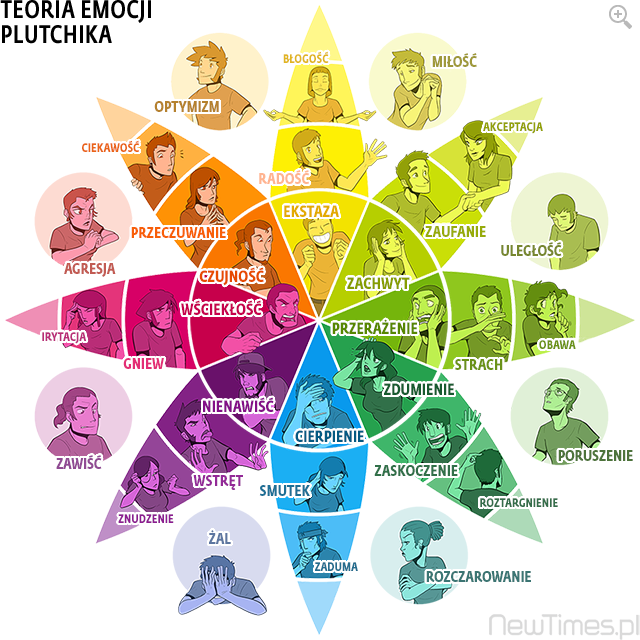
\includegraphics[width=\textwidth]{Plutchik-Emotions-Wheel}
	\caption{Model emocji Plutchika}
	\zrodlo{http://anafora.dmz.edu.pl/teoria-emocji-plutchika/}
	\label{rys:intro:plutnik}
\end{figure}
%http://anafora.dmz.edu.pl/teoria-emocji-plutchika/#jp-carousel-3046
Emocje powstały na drodze ewolucji \cite{Plutchik2001}.
Pozwalają tworzyć błyskawiczne reakcje na bodźce środowiskowe.
Emocje podstawowe tworzą bardziej złożone emocje łącząc się ze sobą.
Emocje znajdujące się naprzeciw siebie nie mogą istnieć w tym samym momencie. 


Ludzie rozpoznają emocje przez odczuwanie. 
Powszechnie stosuje się rozmieszczenie emocji na dwuwymiarowej przestrzeni pobudzenia i wartościowości \cite{Fernandez2004}.
Wysokim poziomem pobudzenia charakteryzują się radość, złość i strach. 
Skutkuje to przyspieszonym biciem serca, podniesionym ciśnieniem krwi, przyspieszonym oddechem, uczuciem suchości w ustach.
Z kolei smutek, będący emocją o niskim pobudzeniu skutkuje spowolnionym biciem serca.
Cechy mowy takie jak częstotliwość podstawowa, dynamika, artykulacja są silnie skorelowane z emocjami o skrajnym pobudzeniu \cite{Cahn1990}.
Pobudzenie nie rozróżnia emocji w sposób wystarczający. 
Przykładowo radość i złość są emocjami o wysokim pobudzeniu, mimo są różnymi emocjami.
Wykorzystywana jest tu cecha emocji zwana wartościowością, określająca, czy dana emocja jest nacechowana pozytywnie czy negatywnie.
Radość jest więc emocją nacechowaną pozytywnie o wysokim pobudzeniu, złość jest nacechowana negatywnie o wysokim pobudzeniu.
Smutek jest emocją negatywną o niskim pobudzeniu.


\section{Ekstrakcja cech}
\subsection{Cechy bazowe}
Rolą cech bazowych jest przetworzenie sygnału czasowego podzielonego na ramki,
do postaci, które zostaną wykorzystane w dalszych etapach obliczeń.
Sygnał w dziedzinie czasu, ma wszystkie informacje, jakie możemy wykorzystać, 
ale analiza sygnału wyłącznie w dziedzinie czasu nie daje zadowalających rezultatów.
Przeniesienie sygnału do dziedziny częstotliwości, przez zastosowanie transformaty Fouriera,
pozwoli analizować jego zmienność w zależności od częstotliwości, 
uzupełniając cechy wyeksponowane w dziedzinie czasu.
\subsubsection{Mel-Frequency Cepstral Coefficients (MFCC)}
Jedną z najpopularniejszych cech wykorzystywanych w systemach automatycznego rozpoznawania mowy,
jest MFCC \ang{Mel-Frequency Cepstral Coefficients}.
Biorąc pod uwagę warunki powstawania mowy, cechy indywidualne mówcy, sposób działania narządów mowy, sposób percepcji mowy przez człowieka,
MFCC daje wektor współczynników reprezentujących mowę z założenia niezależny od mówcy. 
Przekazuje informacje o analizowanym fragmencie mowy, pomijając cechy zależne od mówiącego, takie jak częstotliwość podstawowa i jej harmoniczne \cite{Hossan2013}.
Współczynniki MFC reprezentują dynamiczną naturę mowy, pokazując jej zmianę energii i częstotliwości w czasie.

Algorytm obliczający MFCC przyjmuje na wejście sygnał mowy o długości kilkudziesięciu ms w dziedzinie czasu,
zwracając wektor cech \Rys{rys:mgcc:schemat}.
\begin{figure}[h]
	\centering
	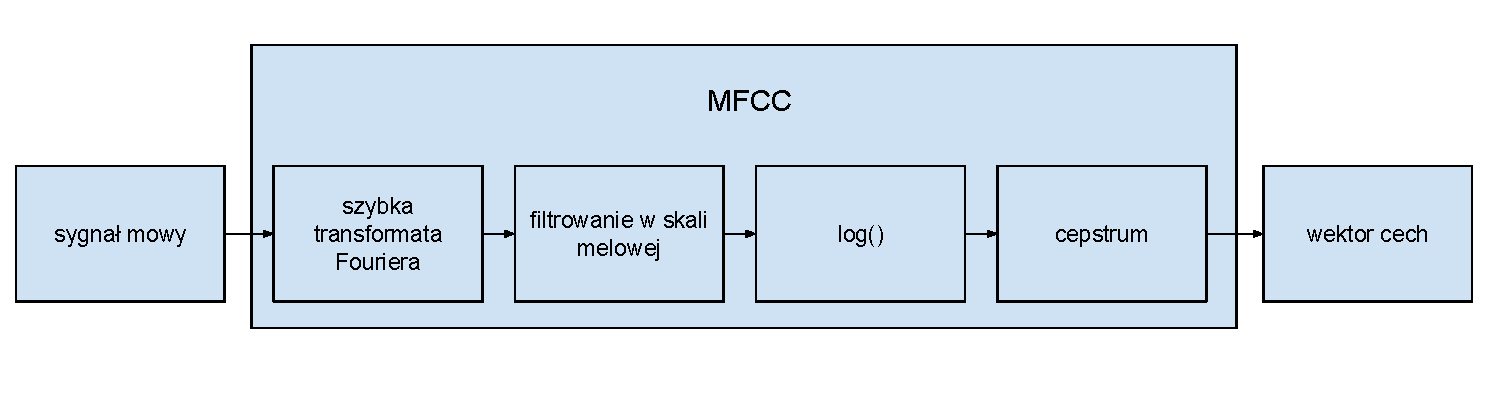
\includegraphics[width=\textwidth]{mfcc-schemat}
	\caption{Algorytm MFCC}
	\label{rys:mgcc:schemat}
\end{figure}

Pierwszym krokiem algorytmu jest obliczenie transformaty Fouriera \cite{Steidl2009}. 
Pozwala ona przenieść sygnał z dziedziny czasu, do dziedziny częstotliwości. 
Operując na sygnale cyfrowym wykorzystana jest dyskretna transformata Fouriera,
\begin{equation}
	X_{k}=\sum _{n=0}^{N-1}x_{n}e^{\frac{-i2\pi kn}{N}}\qquad k=0,\dots ,N-1
\end{equation}, gdzie 
$x_n$ - próbka sygnału czasowego, 
$N$ - liczba próbek w badanym sygnale czasowym,
$X_k$ - próbka sygnału częstotliwościowego.
W praktyce stosuje się wariant szybkiej transformaty Fouriera. 
Szybka transformata Fouriera zwraca podobny wynik, jak dyskretna transformata Fouriera
wykonując znacznie mniej operacji obliczeniowych.

Drugim etapem algorytmu, jest reprezentacja widma w skali melowej. 
Wzorując się na ludzkim narządzie słuchu, 
który postrzega zmianę częstotliwości dźwięku nieliniowo, stosuje się skalę melową.
Skala melowa została zdefiniowana w oparciu o subiektywne odczucia wysokości dźwięku.
Za dźwięk podstawowy przyjmuje się, dźwięk o częstotliwości 1000 Hz i głośności 40 dB wyrażony wartością 1000 melów \cite{KrishnaKishore2013}.
Następnie na podstawie pomiarów i ocen został stworzony wzór
\begin{equation}
	m=2595\log _{10}\left(1+{\frac {f}{700}}\right)
\end{equation}, gdzie
$f$ - częstotliwość w Hz,
$m$ - częstotliwość w melach.
Przeniesienie widma do skali melowej wykonuje się przez aplikację szeregu trójkątnych filtrów środkowoprzepustowych. 
Wprowadza to pewną różnicę, względem psychoakustycznego postrzegania dźwięku, gdzie skala dźwięku jest ciągła.
\begin{figure}[h]
	\centering
	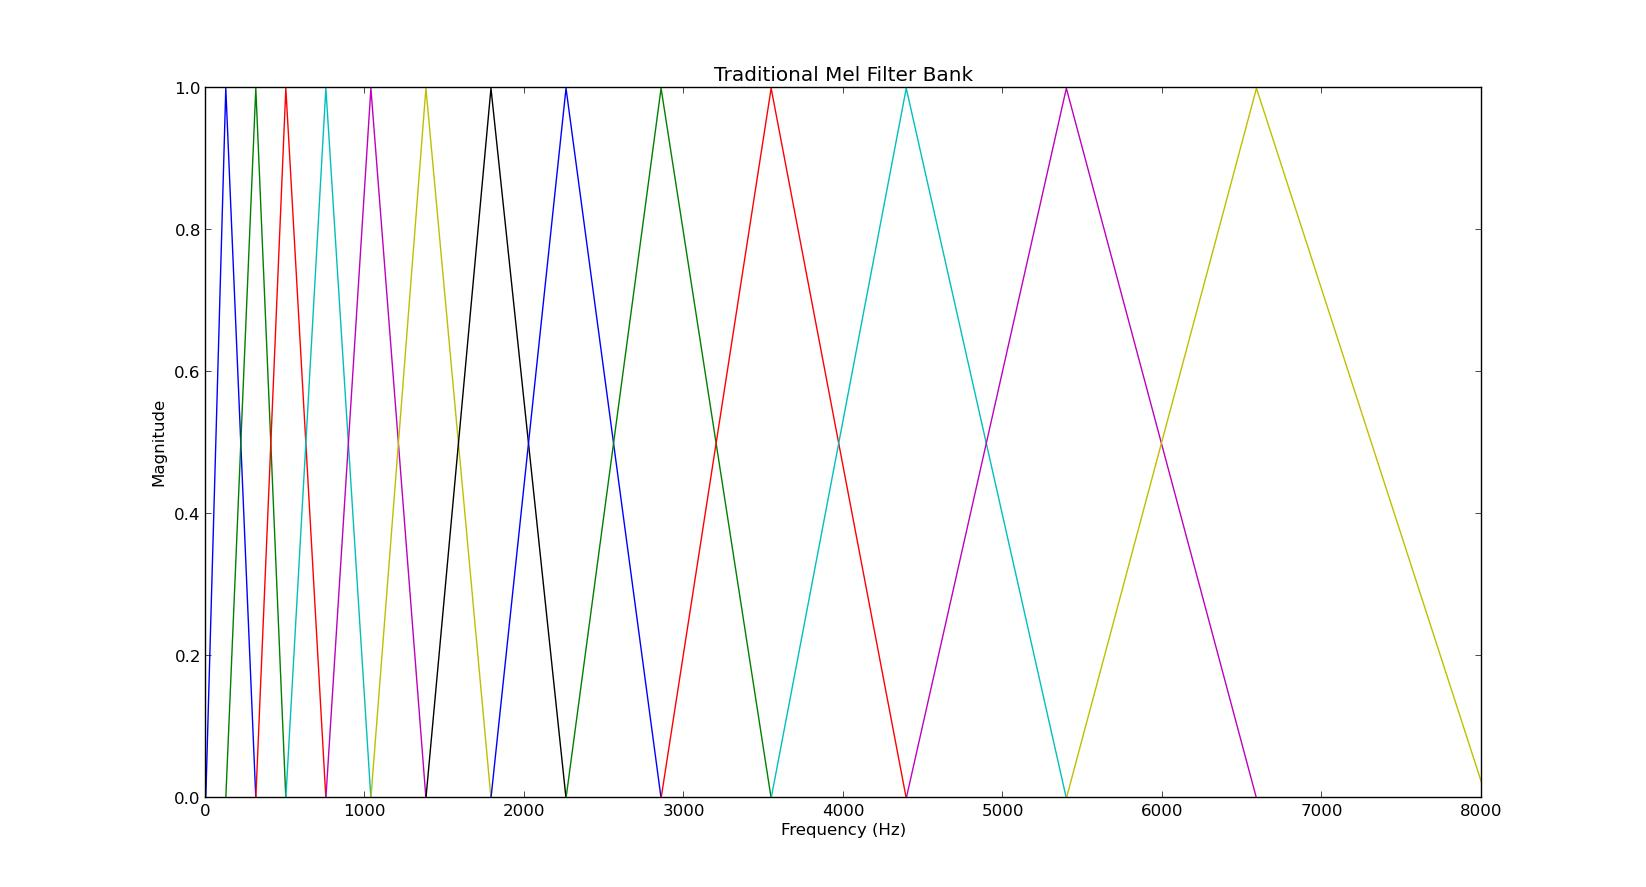
\includegraphics[width=\textwidth]{melfilterbank}
	\caption{Środkowoprzepustowe filtry melowe}
	\zrodlo{https://srohrer32.github.io/eecs351project/}
	\label{rys:mfcc:melfilterbank}
\end{figure}
%https://srohrer32.github.io/eecs351project/

Kolejnym etapem jest obliczenie logarytmu widma w skali melowej.
Odpowiada to interpretacji głośności przez ludzkie ucho,
które odczuwa zmianę głośności w skali logarytmicznej \cite{Hossan2013}.
\begin{equation}
	M'_k=log(M_k)\qquad k=0, \dots, N
	\label{eq:mfcc:log}
\end{equation}
Dla każdej $k$-tej wartości sygnału $M$ jest liczony logarytm, gdzie $N$ jest liczbą wartości w skali melowej \Eq{eq:mfcc:log}.

Ostatnia faza to obliczenie współczynników cepstralnych.
Daje ona odseparowanie sygnału od czynników zależnych od mówcy.
Sygnał głosu zawiera informacje zawarte w komunikacie wypowiedzi oraz 
cechy sygnału zależne od mówcy wynikające z budowy jego narządu mowy oraz sposobu mówienia.
Cechy sygnału zależne od mówcy nie są istotne z punktu widzenia interpretacji przekazu i treści wypowiedzi.
Sygnał w dziedzinie częstotliwości pokazuje wartości energii poszczególnych składowych sygnału.
Przeniesienie sygnału do dziedziny cepstrum pozwala zauważyć częstotliwość zmian sygnału częstotliwościowego.
Zastosowana zostanie dyskretna transformata kosinusowa (DCT-II) \ang{discrete cosine transform} \cite{Hossan2013}.
Dyskretną transformatę kosinusową definiuje wzór:
\begin{equation}
	X_k =
	 \sum_{n=0}^{N-1} x_n \cos \left[k \left(n+\frac{1}{2}\right) \frac{\pi}{N} \right] \quad \quad k = 0, \dots, N-1.
\end{equation}, gdzie
$n$ - numer próbki sygnału czasowego,
$k$ - numer próbki transformaty DCT,
$N$ - liczba próbek w rozpatrywanym sygnale czasowym,
$x_n$ - próbka sygnału czasowego,
$X_k$ - próbka sygnału częstotliwościowego.


\subsubsection{Energia}
Energia sygnału jest sumą kwadratów próbek w ramce.
\begin{equation}
	E_{s}=\sum _{n=-\infty }^{\infty }{|x(n)|^{2}}
	\label{eq:energy}
\end{equation}
Energia sygnału jest wprost proporcjonalna do głośności wypowiedzi.
\subsubsection{Liczba przejść przez zero}
Liczba przejść przez zero \ang{zero crossing rate} znajduje zastosowanie w systemach detekcji mowy.
Pozwala ona stwierdzić, czy w danej ramce występuje mowa \cite{Walters-Williams2010}.
Jest też zależna od częstotliwości tonu. 
Liczbę przejść przez zero wyraża się w liczbie miejsc, gdzie sąsiednie próbki sygnału zmieniły wartość z dodatniej na ujemną lub z ujemnej na dodatnią.
\begin{equation}
	Z = \sum_{n=2}^{N}s(x_n \cdot x_{n-1})\text{, gdzie } s(x) = 
	\begin{cases} 
		0 \text{, dla } x \geq 0 \\
		1 \text{, dla } x < 0
	\end{cases}
	\label{eq:zcr}
\end{equation}
Okresowy sygnał ma niższą liczbę przejść przez zero niż sygnał niezawierający mowy\cite{Walters-Williams2010}.
\subsubsection{Energia}
Entropia mówi o sumie prawdopodobieństw wystąpienia danej wartości próbki $p_k$ w sygnale \cite{Majstorovic2011}.
\begin{equation}
	Ee_{s}=-\sum _{k=1}^{N}p_k log(p_k)
	\label{eq:entropy}
\end{equation}
Jeżeli w ramce występuje wiele skrajnych wartości, entropia sygnału będzie duża. 
Pozwala to stwierdzić zmienność i rozbieżność wartości sygnału w ramce.
\subsubsection{Spectral Subband Centroids (SSC)}
Centroidy Podpasm Widma \ang{Spectral Subband Centroids} opisują cechy widma podobne do formant.
Analizując widmo sygnału dzieli się je na podpasma, następnie znajdując środek ciężkości w każdym podpaśmie \cite{Majstorovic2011}.
\begin{equation}
	C_m=\frac
	{\int_{l_m}^{h_m} f w_m(f) P^\gamma(f)df}
	{\int_{l_m}^{h_m} w_m(f) P^\gamma(f)df}
	\label{eq:ssc}
\end{equation}
Powyższa formuła definiuje centroidy, gdzie dzieląc widmo na $m$ pasm:
\begin{description}
	\item[$C_m$] $m$-ty centroid
	\item[$l_m$] dolna granica pasma
	\item[$h_m$] górna granica pasma
	\item[$w_m$] funkcja filtru
	\item[$P(f)$] moc widma
	\item[$\gamma$] współczynnik mocy widma
\end{description}
Kolejną decyzją jest określenie kształtu filtra środkowoprzepustowego, definiującego pasmo, 
jak i liczbę oraz wzajemnego położenia pasm.
\subsection{Opis statystyczny}
Ostatnim etapem ekstrakcji cech, jest określenie ich parametrów statystycznych.
Dla każdej ramki sygnału zostały obliczone cechy bazowe, opisane w poprzedniej sekcji.
Zostaną one zbadane statystycznie tworząc właściwe cechy, na podstawie których zostanie dokonana klasyfikacja.
Użyto następujących funkcji:
\begin{enumerate}
	\item minimum 
	\item maksimum 
	\item średnia arytmetyczna
	\item wariancja 
	\item skośność
	\item kurtoza
\end{enumerate}
Wykorzystano średnią arytmetyczną, gdzie $N$ jest liczbą ramek, a $x_n$ jest wartością cechy bazowej dla $n$-tej ramki.
\begin{equation}
	\mu = \frac{1}{N}\sum_1^Nx_n
\end{equation}

Skośność - trzeci moment centralny, jest miarą asymetrii rozkładu statystycznego. 
Może przyjąć wartości rzeczywiste.
Intuicyjnie skośność dodatnia oznacza, że lewy ogon rozkładu znajduje się dalej od prawego,
skośność ujemna, że prawy ogon znajduje się dalej,
a zerowa informuje o symetrycznym rozkładzie.
Skośność definiujemy jako
\begin{equation}
	\gamma = E \left [ \left (  \frac{\vec X - \mu}{ \sigma }   \right )^3 \right ]
\end{equation}
gdzie $\mu$ jest średnią arytmetyczną, $\sigma$ odchyleniem standardowym, a $\vec X$ wartościami cechy.

Kurtoza jest czwartym momentem centralnym.
Wyraża spłaszczenie rozkładu. 
Wyrażona jest wzorem
\begin{equation}
	\gamma = E \left [ \left (  \frac{\vec X - \mu}{ \sigma }   \right )^4 \right ]
\end{equation}
gdzie $\mu$ jest średnią arytmetyczną, $\sigma$ odchyleniem standardowym, a $\vec X$ wartościami cechy.
\subsection{Analiza składowych głównych}\label{sec:pca}
Głównym zadaniem selekcji cech jest redukcja wymiarowości obserwacji.
W praktyce, wiele wymiarów jest ze sobą silnie skorelowanych.
Rozważanie obserwacji w skorelowanych wymiarach obniża skuteczność klasyfikacji.
Niektóre klasyfikatory interpretują cechę reprezentowaną przez wiele skorelowanych wymiarów, jako istotniejszą.
Celem selekcji cech, jest wybór takiego zestawu cech, który gwarantuje największą zmienność eliminując wymiary silnie skorelowane, 
lub transformując przestrzeń w sposób gwarantujący największą zmienność w wymiarach.

Analiza składowych głównych - \ang{Principal Component Analysis - PCA} służy redukcji liczby wymiarów przestrzeni,
w których rozpatrywane są obserwacje.
Zmierza do wyboru cech exponujących największą zmienność w zbiorze obserwacji.
Główne składowe zostają uporządkowane w kolejności od największej zmienności do najmniejszej \cite{Bro2014}.
Definiowane są jako wektory własne macierzy kowariancji.

\subsubsection{Standaryzacja}
Do poprawnego działania PCA wymaga ustandaryzowanych danych wejściowych.
Ponieważ PCA ma za zadanie stworzyć podprzestrzeń maksymalizującą wariancję,
należy dane ustandaryzować.
Standaryzacja jest pierwszym etapem PCA.
\subsubsection{Obliczenie wektorów i wartości własnych macierzy kowariancji}
Wartości i wektory własne macierzy kowariancji są podstawą PCA.
Wektory własne określają kierunki nowej przestrzeni cech.
W klasycznym ujęciu PCA polega na rozkładzie na wektory i wartości własne macierzy kowariancji o wymiarach $d \times d$,
gdzie każdy element przedstawia kowariancję pomiędzy dwiema cechami. 
Kowariancję pomiędzy parą cech definiuje się w następujący sposób:
\begin{equation}
	\sigma_{jk}=\frac{1}{n - 1}\sum_{i=1}^{n}(x_{ij}-\bar x_j)(x_{ik} - \bar x_k)
\end{equation}
gdzie 
$n$ - liczba kolumn
$\sigma_{jk}$ - wartość $j,k$ macierzy kowariancji,
$x_{ij}$ - wartość $i,j$ macierzy, 
$\bar{x_j}$ - wartość średnia $j$-tego wiersza,
$x_{ik}$ - wartość $i,k$ macierzy, 
$\bar{x_k}$ - wartość średnia $k$-tego wiersza,

W zapisie macierzowym wzór na macierz kowariancji przedstawia się:
\begin{equation}
	S=\frac{1}{n - 1}\left((\vec{X}-\bar x)^T(\vec{X} - \bar x)\right)
\end{equation}
gdzie $\vec X$ - macierz obserwacji.
Kolejnym krokiem jest znalezienie wartości własnych macierzy kowariancji i odpowiadających im wektorów własnych.
\subsubsection{Sortowanie par wartości i wektorów własnych}
PCA najczęściej jest wykorzystywana do redukcji wymiarowości, 
czyli znalezienia podprzestrzeni, gdzie wektory własne są względem siebie prostopadłe 
i określają osie nowej podprzestrzeni.
W celu określenia, które wektory własne nie wprowadzają istotnej informacji do analizy obserwacji w przestrzeni, bada się odpowiadające im wartości własne.
Wektory własne sparowane z wartościami własnymi o najmniejszych wartościach, 
niosą najmniej informacji o zbiorze. 
Mogą one zostać pominięte w dalszej analizie.
Pary wektorów i wartości własnych są sortowane względem wartości własnych,
te najmniej istotne zostają odrzucone.
W celu określenia, jaka najmniejsza liczba wymiarów pozwoli nam zróżnicować przestrzeń,
wykorzystuje się wyjaśnioną wariancję \cite{Bro2014}.
Wybiera się te wektory własne, które w sumie dają wariancję wystarczająco zbliżoną do wariancji wynikającej ze wszystkich wektorów własnych.

\subsubsection{Macierz projekcji}
Macierz projekcji służy przeniesieniu obserwacji z przestrzeni oryginalnej $d$ wymiarowej,
do przestrzeni $k$-wymiarowej, nie tracąc znaczących informacji.
Do zbudowania macierzy projekcji $\vec W$ posłuży $k$ wektorów własnych posiadających największe własności własne.
\begin{equation}
	W = [\vec e_1 \vec e_2 \dots \vec e_k]
\end{equation}
Ostatnim etapem będzie przeniesienie obserwacji z przestrzeni oryginalnej $X$ do przestrzeni wynikowej $\vec Y = \vec X \times \vec W$.
Liczba wymiarów nowej przestrzeni $d$ jest znacznie mniejsza od liczby wymiarów starej przestrzeni $k$.
\section{Klasyfikacja}
\subsection{Klasyfikator Najbliższych Sąsiadów}
Klasyfikator najbliższych sąsiadów jest prosty w działaniu i implementacji.
Pozwala szybko otrzymać rezultaty, jednak mogą one nie być zadowalające w bardziej złożonych zagadnieniach.
Zasada działania w uproszczeniu sprowadza się do reprezentacji obserwacji za pomocą wektorów cech.
Obliczane są odległości pomiędzy wektorami \cite{Du2013}.
Klasa nowej obserwacji ustalana jest na podstawie klas najbliższych znanych obserwacji ze zbioru uczącego.
Klasyfikator jest podatny na liczbę cech branych pod uwagę w czasie klasyfikacji.
Redukcja liczby parametrów, uwzględniająca usunięcie cech silnie skorelowanych i słabo różnicujących znacząco podnosi wydajność i skuteczność klasyfikatora.

KNN klasyfikuje obserwacje biorąc pod uwagę najbliższą obserwację ze zbioru uczącego.
Obserwacje ze zbioru uczącego rozmieszczone są w wielowymiarowej przestrzeni cech.
Przestrzeń ta jest podzielona na strefy odpowiadające klasom.
Obserwacja znajdująca się w danej strefie zostaje przypisana do klasy, do której ta strefa należy.
Podział na strefy odbywa się w czasie fazy uczenia klasyfikatora.
Kształt i klasa strefy zależy od odległości obserwacji ze zbioru uczącego.
Punkt w przestrzeni przypisany zostaje do danej klasy, jeżeli w jego najbliższym sąsiedztwie zostanie znalezionych $k$ sąsiadów należących do tej klasy.
Należy zdefiniować liczbę $k$ - liczbę wymaganych sąsiadów, pozwalającą określić klasę badanej obserwacji, 
oraz funkcję liczącą dystans pomiędzy dwoma wektorami. Najczęściej jest to norma euklidesowa \cite{Martin2011}.

\begin{algorithm}
	\caption{Klasyfikator Najbliższych sąsiadów}
	\begin{algorithmic}[1]
		\Procedure {kNN}{$T$, $k$, $dist$, $o$}
		\State $D \leftarrow []$
		\ForAll {$t \in T$}
		\State $D(t) \leftarrow dist(t, o)$
		\EndFor
		\State $S \leftarrow sort(D, T)$ \Comment obserwacje posortowane względem odległości
		\State $selectedClass \leftarrow 0$
		\State $counter \leftarrow []$ \Comment licznik najbliższych sąsiadów z klasy
		\Repeat
		\ForAll {$s \in S$}
		\State $counter(class(s))++$
		\EndFor
		\Until{$\neg selectedClass$}
		\EndProcedure
	\end{algorithmic}
	\label{alg:knn:alg}
\end{algorithm}

Dane wejściowe muszą być znormalizowane. 
W przeciwnym razie cechy o bezwzględnie wyższych wartościach będą miały większy wpływ na klasyfikację.
Algorytm \ref{alg:knn:alg} jest wrażliwy na liczbę cech - wymiarów przestrzeni, w której umieszczana jest obserwacja.
Każda cecha odpowiada jednemu wymiarowi w przestrzeni.
Nie jest brana pod uwagę korelacja cech, ani zdolność cech do różnicowania obserwacji.
Dla klasyfikowanej obserwacji obliczany jest dystans pomiędzy tą obserwacją,
a każdą obserwacją ze zbioru testowego.
Prowadzi to do znacznego wzrostu złożoności obliczeniowej klasyfikacji, dla większej liczby cech, czy zbiorów danych uczących.

Istnieją modyfikacje klasyfikatora najbliższych sąsiadów redukujące wymienione wady. 
Opisana została klasyczna wersja algorytmu.

\subsection{Maszyna Wektorów Wspierających (SVM)}

Maszyna Wektorów Wspierających \ang{Support Vector Machine - SVM} wykorzystywana jest do klasyfikacji obserwacji w uczeniu maszynowym.
Należy do grupy modeli uczonych w sposób nadzorowany. 
Uczenie odbywa się przez zadanie zbioru danych testowych, 
każda obserwacja jest oznaczona jako należąca do jednej z dwóch klas.
Algorytm uczący SVM tworzy model rozróżniający obserwacje obydwu klas.
Jako rezultat powstaje klasyfikator binarny, nie probabilistyczny. 

Model powstaje przez rozmieszczenie obserwacji w przestrzeni wielowymiarowej.
Każda obserwacja zostaje umieszczona w $n$-wymiarowej przestrzeni cech i reprezentowana jest przez wektor
zaczynający się w początku układu współrzędnych, a kończący się w punkcie określającym obserwację. 
Hiperpłaszczyzna \ang{hyperplane} jest $n-1$ wymiarowa i zgodnie z definicją rozdziela przestrzeń na dwie części.
Poszukiwana hiperpłaszczyzna powinna być hiperpłaszczyzną optymalną \ang{optimal hyperplane}, 
to znaczy powinna znajdować się w jak największej odległości od najbliższych obserwacji należących do różnych klas \cite{Cortes1995}.

Przestrzeń dwuwymiarową, możemy rozmieścić na płaszczyźnie. 
Prosta dzieli tę płaszczyznę na dwie części.
Analogicznie sytuacja przestawia się w przestrzeni trójwymiarowej.
Może ją przeciąć dowolną płaszczyzną.
Płaszczyzna dzieli przestrzeń trójwymiarową na dwie części, jest więc jej hiperpłaszczyzną.

Sposób tworzenia klasyfikatora SVM jest się następujący.
Obserwacje $x_i$ rozmieszczone są w $n$-wymiarowej przestrzeni cech, gdzie $\vec{x_i} \in R^n$.
Klasy $y_i$ są oznaczone jako $-1$ i $+1$, gdzie $y_i \in \{-1, +1\}$, co można zapisać jako:
\begin{equation}
	(\bm{x_1},y_1), ..., (\bm{x_i}, y_i), \textrm{ gdzie } y_i \in \{-1, +1\}
\end{equation}

Obserwacje są liniowo separowalne, jeżeli istnieje wektor $\bm{w}$ i taki skalar $b$, że nierówności
\begin{gather}
	\bm{w} \cdot \bm{x_i} + b \geq 1 \textrm{ jeśli } y_i = 1\\
	\bm{w} \cdot \bm{x_i} + b \leq 1 \textrm{ jeśli } y_i = -1,
\end{gather}
są prawdziwe dla wszystkich obserwacji w zbiorze \cite{Cortes1995}.
Powyższy układ nierówności można zapisać w postaci:
\begin{equation}
	y_i(\bm{w} \cdot \bm{x_i} + b) \geq 1
\end{equation}
Hiperpłaszczyzna optymalna 
\begin{equation}
	\bm{w_0} \cdot \bm{x_i}  + b_0 = 0
\end{equation}
istnieje w przypadku, kiedy rozdziela zbiór treningowy z zachowaniem największej możliwej odległości od obserwacji obydwu klas.
Odległość pomiędzy obserwacjami a hiperpłaszczyzną definiuje
rzut skalarny \ang{scalar projection} \Eq{svm:eq:rzut} wektora obserwacji $\bm{x}$ na wektor jednostkowy $\hat{\bm{w}} = \frac{\bm{w}}{|\bm{w}|}$
obrazujący położenie płaszczyzny.
\begin{equation}
	\rho(\bm{w}, b) = \min\limits_{\{x:y=1\}} \frac{\bm{x} \cdot \bm{w}} {|\bm{w}|} - \max\limits_{\{x:y=-1\}}  \frac{\bm{x} \cdot \bm{w}} {|\bm{w}|} 
	\label{svm:eq:rzut}
\end{equation}
Wartość rzutu skalarnego jest odległością obserwacji od hiperpłaszczyzny. 
Różnica najmniejszej odległości pomiędzy hiperpłaszczyzną a obserwacją należącą do klasy $y=1$
oraz największej odległości pomiędzy hiperpłaszczyzną a obserwacją należącą do klasy $y=-1$ 
powinna być jak największa.
Obserwacje znajdujące się w najmniejszej odległości od hiperpłaszczyzny nazywane są wektorami wspierającymi \ang{support vectors}

Klasyfikacja polega na umieszczeniu klasyfikowanej obserwacji w przestrzeni cech.
Obserwacja należy do tej klasy, do której należą obserwacje leżące po tej samej stronie hiperpłaszczyzny.
\subsubsection{Uczenie}
%http://fourier.eng.hmc.edu/e161/lectures/svm/node3.html
Uczenie odbywa się przez zadanie zbioru obserwacji testowych. 
Mamy zbiór obserwacji, separowalny liniowo, każda z obserwacji $\vec{x}_k$ należy do klasy $-1$ lub $1$:
\begin{equation}
	\{ ({\bf x}_k, y_k), k=1,\cdots,K \} \mbox{, gdzie } y_k \in \{1,-1\}
\end{equation}
Celem optymalizacji jest odnalezienie wektora $\vec{w}$ i stałej $b$ wyznaczających hiperpłaszczyznę
sperarującą liniowo obserwacje różnych klas w przestrzeni. 

Weźmy wektor początkowy $\vec{w} = 0$ i zbiór danych uczących $K$.
Obliczamy pierwszą wartość wektora $\vec{w}$
\begin{equation}\label{eq:svm:hyperplane}
	{\vec{w}}=\sum_{i=1}^K \alpha_i y_i {\vec{x}}_i
\end{equation}
gdzie $\alpha_i>0$ \cite{Mittal2016}.
Podczas każdego cyklu uczącego, wektor $\vec{w}$ może zostać zmodyfikowany przez obserwację, 
zgodnie z regułą:
\begin{equation}
	\mbox{jeżeli } y_i f({\vec{x}}_i)=y_i ({\vec{x}}_i^T{\vec{w}}^{stary}+b)
	=y_i\left(\sum_{j=1}^m \alpha_j y_j({\vec{x}}_i^T{\vec{x}}_j)+b\right)<0,
\end{equation}
\begin{equation}
	\mbox{to } {\vec{w}}^{nowy}={\vec{w}}^{stary}+\eta y_i {\vec{x}}_i
	=\sum_{j=1}^{m} \alpha_j y_j\vec{x}_j +\eta y_i {\vec{x}}_i,
\end{equation}
\begin{equation}
	\mbox{np. }
	\alpha_i^{nowy}=\alpha_i^{stary}+\eta
\end{equation}
gdzie $0 < \eta < 1$ jest parametrem uczenia.
Ostatecznie płaszczyznę \Eq{eq:svm:hyperplane} określamy dobierając wartości $\alpha_i$ według zależności: 
\begin{equation}
	\mbox{jeżeli } y_i\left(\sum_{j=1}^m \alpha_j y_j({\vec{x}}_i^T\vec{x}_j)+b\right)<0,
	\mbox{to } \alpha_i^{new}=\alpha_i^{old}+\eta 
\end{equation}

\subsubsection{Hiperpłaszczyzna Miękkiego Marginesu}
Obserwacje rozmieszczone w przestrzeni wielowymiarowej nie są separowalne liniowo. 
Rozwiązanie problemu nieseparowalnego liniowo sprowadza się do znalezienia hiperpłaszczyzny Miękkiego Marginesu \ang{Soft Margin}, 
która rozdziela obserwacje dwóch klas zawierającą jak najmniejszą liczbę błędnych klasyfikacji.
W takim przypadku błędne klasyfikacje są nie do uniknięcia \cite{Dellepiane2015}.
Poszukiwanie rozwiązania polega na wyznaczeniu hiperpłaszczyzny rozdzielającej przestrzeń 
minimalizując błędy klasyfikacji na zbiorze uczącym i nieznanym zbiorze testowym.

Przyjmijmy zbiór uczący $D$, który nie jest separowalny liniowo. 
Nie istnieje hiperpłaszczyzna rozdzielająca obserwacje dwóch klas.
Zostanie więc stworzony margines błędu, dopuszczający istnienie błędnych klasyfikacji w swoim obrębie.
Występowanie błędnych klasyfikacji jest tolerowane, ale wystąpienia błędnych klasyfikacji są minimalizowane.
Błędną klasyfikację wyraża się zmienną pomocniczą $\xi_i$ \ang{slack variable}. 
Wartość zmiennej pomocniczej $\xi_i$ jest wprost proporcjonalna do odległości obserwacji $\vec{x_i}$
Formalnie problem optymalizacji SVM można zapisać w postaci:

\begin{equation}
\mbox{zminimalizuj } {\vec w}^T {\vec w}+C\sum_{i=1}^m \xi_i^k
\end{equation}
%http://fourier.eng.hmc.edu/e161/lectures/svm/node2.html

\begin{equation}
	\mbox{zakładając, że }  y_i ({\bf x}_i^T {\bf w}+b) \ge 1-\xi_i,
	\mbox{, }x_i \ge 0 \mbox{, }(i=1,\cdots,m)
\end{equation}
Parametr $C$ steruje maksymalizacją marginesu i minimalizacją błędów uczenia.
Jeżeli parametr $C$ ma małą wartość, margines dopuszcza zbyt wiele błędów klasyfikacji.
Duża wartość parametru $C$ może skutkować przeuczeniem modelu.
Parametr $k$ określa normę marginesu. 
Margines pierwszej normy jest mniej wrażliwy na obserwacje leżące poza nim,
dzięki temu margines pierwszej normy jest lepszy do klasyfikacji danych mniej uporządkowanych.

\subsubsection{Funkcje jądra}
Funkcja jądra \ang{kernel method} 
przyporządkowuje każdej reprezentacji obserwacji w przestrzeni,
reprezentację w innej przestrzeni o większej liczbie wymiarów.
Zabieg zwiększenia liczby wymiarów ma na celu ułatwienie 
klasyfikacji, czy klasteryzacji zbioru danych względem
reprezentacji w przestrzeni pierwotnej. 

Przykładem jest SVM, poszukujący hiperpłaszczyzny.
Jeżeli dane nie są seprowalne liniowo,
ale są separowalne nieliniowo to stosując sztuczkę jądra \ang{kernel trick} 
przeniesiemy zbiór obserwacji do przestrzeni w której będzie on separowalny liniowo \cite{Patle2013}.

\begin{equation}
	\langle \vec{x_1} \cdot \vec{x_2} \rangle \gets K(\vec{x_1}, \vec{x_2}) = \langle \Phi(\vec{x_1}) \cdot \Phi(\vec{x_2}) \rangle
\end{equation}

Jądro liniowe \Eq{eq:svm:kern:lin} jest najprostszą funkcją jądra. 
sprowadza się do iloczynu wektorowego i dodania stałej $c$.
Liniowa funkcja jądra w niektórych przypadkach nie wprowadza zmian zmieniających rezultat działania algorytmu.
\begin{equation}
	\label{eq:svm:kern:lin}
	K(\vec x, \vec{x_i}) = \vec x \cdot \vec x ^ T + c
\end{equation}

Wielomianową funkcję jądra określają współczynnik $\alpha$, stałą $c$ i stopień wielomiany $d$.
\begin{equation}
	\label{eq:svm:kern:poly}
	K(\vec x, \vec{x_i}) = (\alpha \vec x^T \vec x_i + c)^d 
\end{equation}

Jądro sigmoidalne \Eq{eq:svm:kern:sig} pochodzi z dziedziny sieci neuronowych,
gdzie funkcjonuje sigmoidalna funkcja aktywacji neuronu. 
Model SVM z sigmoidalną funkcją jądra jest równoważny dwuwarstwowej perceptonowej sieci neuronowej.
Posiada dwa parametry: współczynnik $\alpha$ i stałą $c$, gdzie zazwyczaj $c$ przyjmuje wartość $1/N$,
dla $N$-wymiarowej przestrzeni.
\begin{equation}
	\label{eq:svm:kern:sig}
	K(\vec{x_i}, \vec{x_j}) = tanh( \alpha \vec{x_i}  \vec{x_j} + c)
\end{equation}
%http://crsouza.com/2010/03/17/kernel-functions-for-machine-learning-applications/
\subsection{Sztuczne sieci neuronowe}
Sztuczne sieci neuronowe \ang{Artificial Neural Network} są modelami zainspirowanymi ludzkim mózgiem.
Składają się z ogromnej liczby węzłów, każdy węzeł wykonuje prostą operację matematyczną.
Każdy neuron posiada wejścia, wyjście oraz zestaw parametrów go określających. 
Dzięki połączeniom węzłów (sztucznych neuronów) sieci neuronowe są w stanie rozwiązywać złożone problemy.
Proces uczenia sieci neuronowej polega na dostosowywaniu parametrów węzłów prowadzącego do znalezienia optymalnego rozwiązania problemu.
Sztuczne sieci neuronowe są bardzo popularnym i rozbudowanym zagadnieniem uczenia maszynowego.
Znajdują zastosowanie w rozpoznawaniu obrazów, mowy, pisma, robotyce. 

\subsubsection{Model neuronu}
Ludzki mózg jest złożony z ok $10^{11}$ neuronów.
Odbierają one sygnały od innych neuronów, do których są podłączone.
Na podstawie wejścia decydują, czy podać sygnał na wejście.
Pojedynczy neuron nie rozwiązuje złożonych problemów.
Wiele neuronów połączonych w sieć jest w stanie wykonać skomplikowane operacje matematyczne.
Pojedynczy neuron składa się z wejścia $\vec{x}$, wyjścia $y$, wektora wag $\vec{w}$ i przesunięcia $b$ \ang{bias}.
Decyzję o podaniu sygnału na wyjście podejmuje funkcja aktywacji $g(\vec{x} \cdot \vec{w} + b)$.
Wyjściem neuronu są liczby z przedziału $(0, 1)$.
Na potrzeby tej sekcji przyjmijmy progową funkcję aktywacji $g(x)$ \Eq{eq:mlp:step}.
\begin{equation}
	\label{eq:mlp:step}
g(x)={\begin{cases}0{\text{, dla }}x<0\\1{\text{, dla }}x\geq 0\end{cases}}
\end{equation}
Neutron przyjmuje na wejście wektor $\vec{x}$.
Wektor wejściowy zostaje pomnożony przez wektor wag $\vec{w}$ i dodany do progu aktywacji $b$.
Rezultat jest argumentem funkcji aktywacji  $g(\vec{x} \cdot \vec{w} + b)$.
Wartość funkcji aktywacji zostaje podana na wyjście. \Rys{rys:mlp:neuron}.
Możliwości pojedynczego neuronu są ograniczone \cite{Jeon2018}.
Posiada jedynie wyjście binarne zwracające $0$ lub $1$. 
Zadaniem neuronu jest określenie, po której stronie hiperpłaszczyzny, 
określonej przez wektor $\vec w$ i skalar $b$ znajduje się obserwacja.
Funkcja aktywacji ogranicza odpowiedź do wcześniej zadanego zakresu.
\begin{figure}[h]
	\centering
	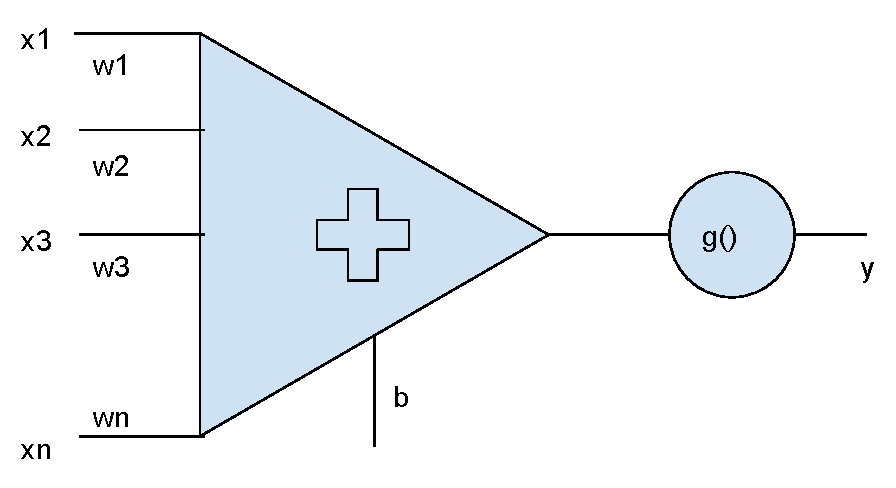
\includegraphics[width=\textwidth]{neuron}
	\caption{Schemat neuronu}
	\label{rys:mlp:neuron}
\end{figure}

\subsubsection{Funkcja aktywacji}
Funkcja aktywacji określa odpowiedź neuronu.
Co do zasady neuron zwraca odpowiedź binarną \textit{wszystko albo nic}.
Przykładem jest skokowa funkcja aktywacji \Eq{eq:mlp:step}.
\begin{figure}[h]
	\label{wyk:mlp:step}
	\centering
	\begin{gnuplot}[terminal=pdf,terminaloptions=color]
		set xrange [-1:1] 
		set yrange [-.5:1.5]
		step(x) = x>0 ? 1 : 0
		plot step(x)
	\end{gnuplot}
	\begin{equation}
		step(x)={\begin{cases}0{\text{, dla }}x<0\\1{\text{, dla }}x\geq 0\end{cases}}
	\end{equation}
	\caption{Progowa funkcja aktywacji}
\end{figure}

W praktyce stosuje się funkcje ciągłe, dające wartość z zakresu od $0$ do $1$.
Najczęściej spotykaną ciągłą funkcją logiczną jest funkcja sigmoidalna.
Może przyjąć wszystkie wartości z zakresu $y \in (0,1)$.
Rzutuje to na interpretację wartości zwracanej przez neuron,
która nie działa już zgodnie z regułą \textit{wszystko, albo nic}.
Neuron z funkcją sigmoidalną nie jest już klasyfikatorem binarnym, ponieważ może zwrócić np. wartość $sigm(0) = 0,5$.
Pozwala to na tworzenie sieci neuronowych operujących na rozmytej,
zwiększając zakres problemów w których zastosowanie mogą znaleźć sztuczne sieci neuronowe.

%http://lowrank.net/gnuplot/datafile2-e.html

\begin{figure}[h]
	\label{wyk:mlp:sigm}
	\centering
	\begin{gnuplot}[terminal=pdf,terminaloptions=color]
		set xrange [-10:10] 
		set yrange [-.5:1.5]
		sigm(x) = 1/(1+exp(-x))
		plot sigm(x)
	\end{gnuplot}
	\begin{equation}
		sigm(x)=\frac{1}{1+e^{-x}}
	\end{equation}
	\caption{Sigmoidalna funkcja aktywacji}
\end{figure}
\subsubsection{Schemat i zasada działania sztucznej sieci neuronowej}
Sieć neuronowa zbudowana jest z wielu neuronów połączonych ze sobą.
Wyjścia jednych neuronów przekazywane są jako wejścia dla kolejnych.
Schemat budowy sieci neuronowej można przedstawić za pomocą grafu skierowanego \Rys{rys:mlp:graf}.
\begin{figure}[h]
	\centering
	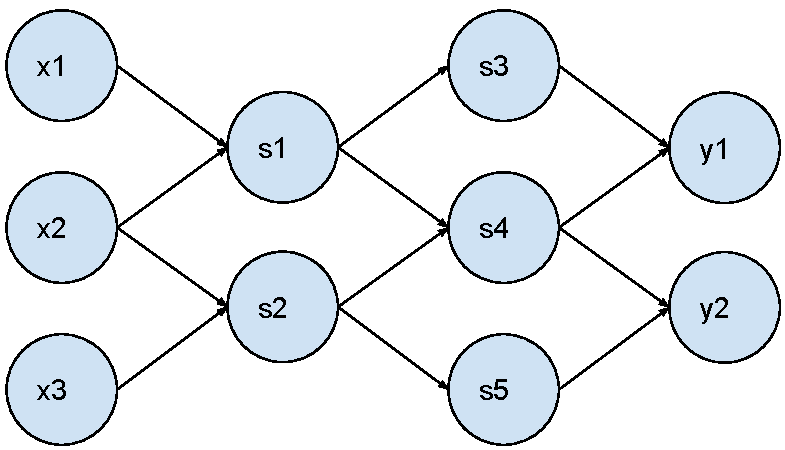
\includegraphics[width=\textwidth]{ann-graf}
	\caption{Sieć neuronowa jako graf}
	\label{rys:mlp:graf}
\end{figure}
Węzły grafu oznaczają neurony, a krawędzie wagi wejść neuronów, do których prowadzą.
Wyjścia jednych neuronów są wejściami dla drugich.
Wyróżniamy dwa typy sieci neuronowych.
Sieci neuronowe jednokierunkowe, w reprezentacji grafowej tworzą acykliczny graf skierowany.
Dzięki wyeliminowaniu cykli z sieci jej reprezentacja, uczenie i obliczenia zostają w znacznej mierze uproszczone. 
Sieci neuronowe, w których występują cykle, nazywane są sieciami rekurencyjnymi.
Węzły $x_1$ i $x_2$ są wejściami sieci neuronowej.
Węzły $s_{1..5}$, $y_1$ i $y_2$ są neuronami z funkcją aktywacji.
Wartości wyjściowe z węzłów $y_1$ i $y_2$ są wyjściami całej sieci neuronowej \cite{Gurgen2017}.
Przykładowo wejście $x_1$ zostaje pomnożone przez wagę $w_{x_1s_1}$ i staje się pierwszym wejściem dla neuronu $s_1$, itd.

Stosuje się logiczny podział węzłów na warstwy \Rys{rys:mlp:warstwy}.
Warstwa $L_0$ nazywana jest warstwą wejściową.
Przyjmuje ona wektor $\vec x$, który jest przetwarzany w kolejnych warstwach.
Warstwy $L_1$ i $L_2$ są warstwami ukrytymi sieci. 
Wartości przyjmowane i zwracane przez neurony warstw ukrytych nie są widoczne z zewnątrz sieci.
W sieciach jednokierunkowych każda warstwa zależy wyłącznie od wartości z warstwy poprzedniej.
Wartości zwrócone przez warstwę $L_3$ - wyjściową są wynikiem działania całej sieci neuronowej.
\begin{figure}[h]
	\centering
	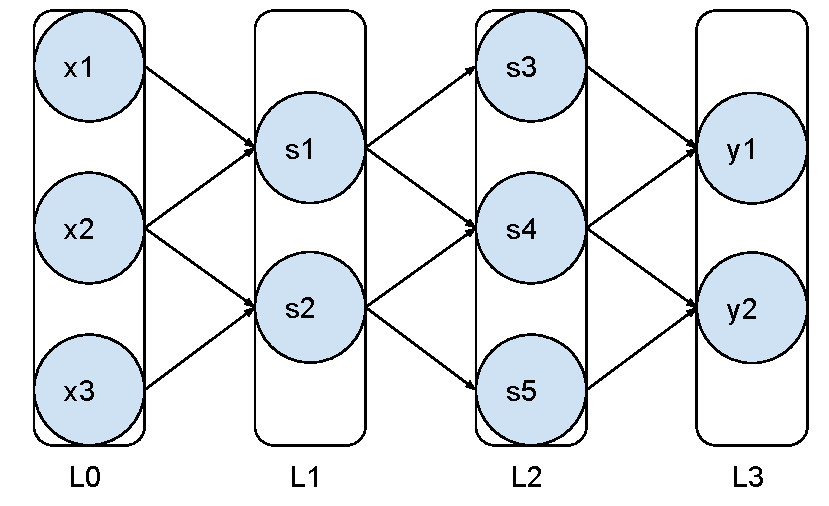
\includegraphics[width=\textwidth]{ann-warstwy}
	\caption{Warstwy sieci neuronowej}
	\label{rys:mlp:warstwy}
\end{figure}
\subsubsection{Percepton wielowarstwowy - MLP}
Percepton wielowarstwowy \ang{Multi-layer percepton} jest najpopularniejszym typem sztucznej sieci neuronowej.
Jest zbudowany z warstw wejściowej, wyjściowej i wielu warstw ukrytych.
Percepton wielowarstwowy w odróżnieniu od perceptonu jednowarstwowego może rozwiązywać problemy nieliniowe.
Przykładem funkcji, której nie może zamodelować pojedynczy percepton jest XOR \ang{exclusive or} \Tab{tab:mlp:xor}.
\begin{table}[h]
	\centering
	\begin{tabular}{ |l|c|r| }
		\hline
		$x_1$	& $x_2$& $XOR$ \\ \hline
		0 	& 0 	& 0 \\ \hline
		0 	& 1 	& 1 \\ \hline
		1 	& 0 	& 1 \\ \hline
		1 	& 1 	& 0 \\ \hline
	\end{tabular}
	\caption{Tabela funkcji XOR}
	\label{tab:mlp:xor}
\end{table}
Wykres \ref{wyk:mlp:xor} obrazuje funkcję $XOR$ oraz przykładowe hiperpłaszczyzny.
Nie istnieje hiperpłaszczyzna rozdzielająca argumenty, dla których wartość $XOR$ przyjmuje $1$,
od argumentów, dla których $XOR$ przyjmuje wartość $0$ \cite{Labib2010}.
\begin{figure}[h]
	\label{wyk:mlp:sigm}
	\centering
	\begin{gnuplot}[terminal=pdf,terminaloptions=color]
		set xrange [-1:2]
		set yrange [-1:2]
		linia1(x)=x+.5
		linia2(x)=-2*x+1.5
		plot "-" using 1:2 title 'XOR(x1, x2)=1',\
		"-" using 1:2  title 'XOR(x1, x2)=0',\
		linia1(x),\
		linia2(x)
		0	1
		1	0
		end
		0	0
		1	1
		end
	\end{gnuplot}
	\caption{Wykres XOR}
	\label{wyk:mlp:xor}
\end{figure}
Percepton wielowarstwowy dzięki zastosowaniu wielu warstw ukrytych, 
jest w stanie zróżnicować zbiory, które nie są separowalne liniowo.
\chapter{Struktura oprogramowania}
Zasadniczą częścią pracy, jest napisanie programu komputerowego zdolnego rozróżnić emocje mówcy na podstawie dźwiękowego zapisu wypowiedzi.
Aplikacja została zaimplementowana w języku \textit{Python}. 
Została podzielona na dwie części. 
Pierwsza część aplikacji odpowiada za ekstrakcję cech sygnału z plików audio,
druga dokonuje klasyfikacji emocji na podstawie wcześniej określonych cech.

Opis środowiska:
\begin{description}
	\item [system operacyjny] Debian 8.10 Jessie stabilny 
	\item [wersja jądra] 3.16.0-4-amd64
	\item [Python] 2.7.9
	\item [numpy] 1.13.3
	\item [scikit-learn] 0.19.1
	\item [python-speech-features] 0.6
\end{description}
Python jest interpretowanym, obiektowo zorientowanym, dynamicznie typowanym językiem programowania.
Operuje na wysokopoziomowych strukturach, których typy i zależności są rozwiązywane dynamicznie.
Jako język elastyczny jest przeznaczony do szybkiego tworzenia aplikacji, skryptów, czy integracji istniejących komponentów.
Python charakteryzuje się prostą składnią sterowaną białymi znakami 
(np. zamiast nawiasów klamrowych znanych z C, czy Javy, Python wykorzystuje wcięcia w kodzie definiując bloki kodu).
Podejście to wymusza pisanie bardziej czytelnego kodu.
Kod jest dzielony na moduły i pakiety.
Python posiada duży zbiór bibliotek rozwijanych przez społeczność.

Numpy to najpopularniejsza biblioteka wykorzystywana do obliczeń numerycznych i uczenia maszynowego.
Pozwala operować na n-wymiarowych macierzach, zawiera podstawowe funkcje algebry liniowej itd.
\\
Scikit-learn jest biblioteką dostarczającą wymagane przez współczesny stan wiedzy implementacje algorytmów uczenia maszynowego.
Docelowo znajduje zastosowanie przy rozwiązywaniu zadań statystycznych, analitycznych i eksploracji danych \cite{OShaughnessy2008}.  
\\
Python-speech-features to niewielka biblioteka wspierająca systemy automatycznego rozpoznawania mowy. 
Dostarcza implementacje MFCC i SSC.
\chapter{Przeprowadzone badania}
\section{Opis bazy danych}\label{sec:opis_bazy_danych}
W pracy wykorzystano bazę danych emocji w mowie powstałą w Akademii Górniczo-Hutniczej w Krakowie.
Nagrania zawierają pięć emocji podstawowych: radość, smutek, złość, strach, zdziwienie.
Ponadto zostały nagrane wypowiedzi w tonie neutralnym jako punkt odniesienia i ironicznym, jako emocja złożona.
W nagraniu wzięło udział 6 mężczyzn i 6 kobiet w wieku od 20 do 30 lat. 
Mówcy byli zarówno profesjonalnymi aktorami jak i amatorami, czy wolontariuszami.
Baza została zrealizowana jako baza danych emocji odgrywanych. 

Nagrano 4 typy wypowiedzi.
\begin{description}
	\item [Zdania] będące sekwencją 46 prostych wypowiedzi często wykorzystywanych w życiu codziennym 
		np. ,,Dzień dobry'', ,,Witam serdecznie''. 
	\item [Polecenia]  np. ,,Nowy'', ,,Otwórz''. 
		Jest to głosowa reprezentacja standardowych komend wykorzystywanych w komunikacji człowieka z komputerem.
	\item [Cyfry] od 0 do 9.
	\item [Tekst] czyli fragment artykułu. 
		Lity tekst będący spójnym logicznie ciągiem zdań, lecz wyrwanym z kontekstu.
\end{description}
Dla każdego z 6 mówców zarejestrowano każdy typ wypowiedzi we wszystkich stanach emocjonalnych.

Baza danych składa się z opisu oraz wypowiedzi posegregowanych w katalogach oznaczających odgrywaną emocję.
Nazwy plików wskazują na mówcę, emocję oraz typ wypowiedzi.
Nagrania zostały zapisane w formie plików WAV przy częstotliwości próbkowania 44100Hz i rozdzielczości 16 bitów ~\cite{Igras2009}.

Nagrania nie zostały poddane przetwarzaniu wstępnemu. 
Różnią się poziomem głośności.
Pojedyncze nagrania wyglądają na ustandaryzowane, ale stanowią wyjątek.
Dokładna historia nagrań nie jest znana, ich stan jest niejednolity.
Brak jest informacji o operacjach wykonywanych na nagraniach.
Stan nagrań jest niejednorodny i nieznany.
\begin{figure}[h]
	\centering
	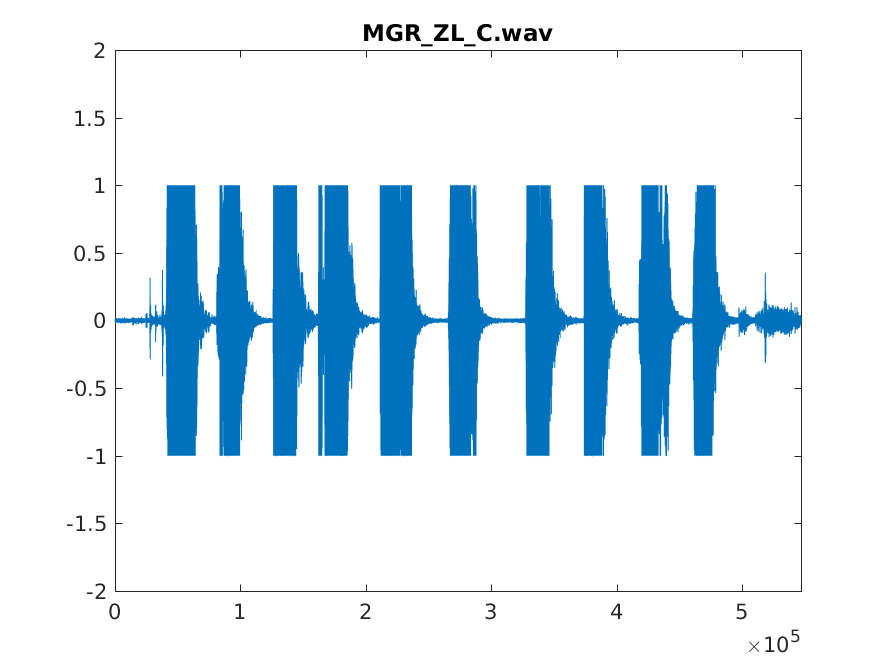
\includegraphics[width=\textwidth]{MGR_ZL_C-plot}
	\caption{Przykład ustandaryzowanego sygnału}
	\label{rys:opis:ustandaryzowany}
\end{figure}
\begin{figure}[h]
	\centering
	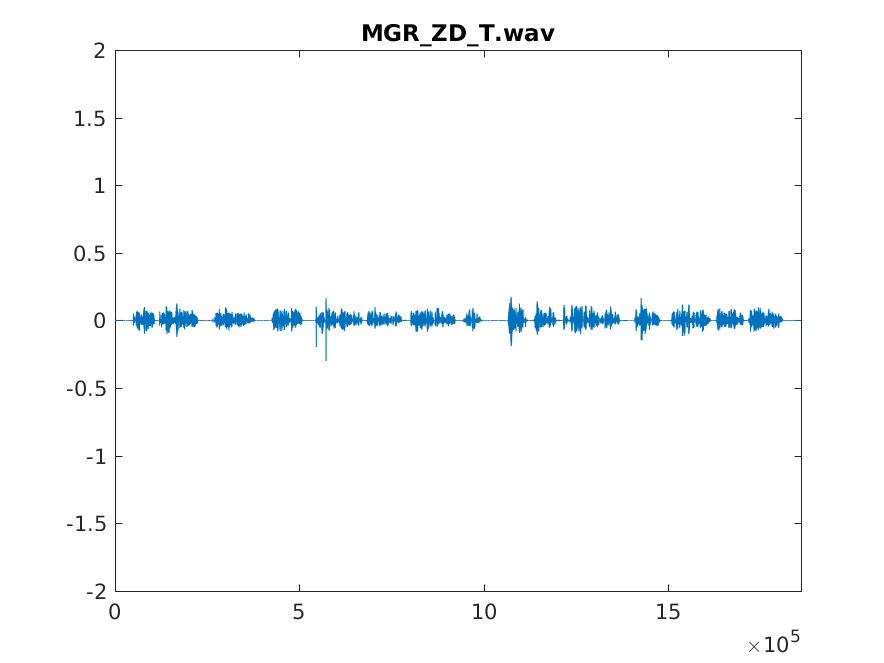
\includegraphics[width=\textwidth]{MGR_ZD_T-plot}
	\caption{Przykład nie ustandaryzowanego sygnału}
	\label{rys:opis:nieustandaryzowany}
\end{figure}

Zapis wypowiedzi został ustandaryzowany\Rys{rys:opis:ustandaryzowany} w celu zniwelowania różnic wynikających z głośności nagrania\Rys{rys:opis:nieustandaryzowany}.
\section{Ekstrakcja cech wypowiedzi}
Ekstrakcja cech rozpoczyna się od znalezienia w bazie danych wszystkich plików zwierających wypowiedź i~odczytania sygnału. 
Nie rozróżniano wypowiedzi ze względu na ich treść: polecenia, zdania, cyfry, tekst.
Kolejnym krokiem jest przetwarzanie wstępne. 
Sygnały stereofoniczne sumowane są do monofonicznych, sygnał zostaje poddany standaryzacji.
W następnym etapie sygnał dzielony jest na ramki o długości 500ms zachodzące na siebie co 200ms.
Z przetworzonego wstępnie i podzielonego na ramki sygnału obliczane są cechy sygnału \Lst{lst:res:extr}.
\begin{lstlisting}[language=Python,label={lst:res:extr},caption={funkcja obliczająca cechy sygnału pojedynczego pliku}]
def analyse_file(filename):
    f = read_file(filename)
    p = preprocess(f)
    frames = split(p, 500, 200)
    features = [extract_features(frame) for frame in frames]
    feturesMap = features_to_map(features)
    return statistical_describe_features(feturesMap)
\end{lstlisting}
Dla każdej ramki policzono zestaw cech podstawowych: 
\begin{itemize}
	\item MFCC
	\item energię
	\item liczba przejść przez zero
	\item energię entropii
	\item SSC.
\end{itemize}
Następnie dla każdej cechy podstawowej dla wszystkich ramek obliczono wartości:
\begin{itemize}
	\item minimalną
	\item maksymalną
	\item średnią
	\item kurtozę
	\item skośność
	\item wariancję
\end{itemize}
Wyniki obliczeń są zapisane w formacie CSV.
Pojedynczy rekord zawiera informacje o nazwie pliku, zarejestrowanej na nim emocji, 
oraz wartościach obliczonych cech.
Cechy zostały nazwane w konwencji \textit{(cecha bazowa) (numer wartości w wektorze) (statystyka)}.
Przykładowo wartości \textit{mfcc 1 min}, \textit{ssc 20 max}, \textit{ssc 24 max}, \textit{mfcc 3 kurtosis} oznaczają kolejno:
\begin{itemize}
\item wartość najmniejszą pierwszej wartości wektora cech MFCC
\item wartość największą dwudziestej wartości wektora cech SSC
\item wartość największą dwudziestej czwartej wartości wektora cech SSC
\item kurtozę trzeciej wartości wektora cech MFCC
\end{itemize}
Dane zostają zapisane w pliku $features_analysis.csv$ w celu dalszego przetwarzania.
Wyznaczono wartości następujących cech:
\begin{itemize}
\item energia kurtoza
\item energia wartość maksymalna
\item energia średnia
\item energia wartość minimalna
\item energia skośność
\item energia wariancja
\item entropia kurtoza
\item entropia wartość maksymalna
\item entropia średnia
\item entropia wartość minimalna
\item entropia skośność
\item entropia wariancja
\item MFCC (współczynniki 1-13)  kurtoza
\item MFCC (współczynniki 1-13)  wartość maksymalna
\item MFCC (współczynniki 1-13)  średnia
\item MFCC (współczynniki 1-13)  wartość minimalna
\item MFCC (współczynniki 1-13)  skośność
\item MFCC (współczynniki 1-13)  wariancja
\item SSC (współczynniki 1-26)  kurtoza
\item SSC (współczynniki 1-26)  wartość maksymalna
\item SSC (współczynniki 1-26)  średnia
\item SSC (współczynniki 1-26)  średnia
\item SSC (współczynniki 1-26)  wartość minimalna
\item SSC (współczynniki 1-26)  skośność
\item SSC (współczynniki 1-26)  wariancja
\item liczba przejść przez zero kurtoza
\item liczba przejść przez zero wartość maksymalna
\item liczba przejść przez zero średnia
\item liczba przejść przez zero wartość minimalna
\item liczba przejść przez zero skośność
\item liczba przejść przez zero wariancja
\end{itemize}

\section{Klasyfikacja emocji}
Klasyfikacja emocji została przeprowadzona na wcześniej przygotowanej bazie cech.
Cechy rozmieszczone w przestrzeni zostały poddane redukcji wymiarowości. 
Skorelowane cechy nie różnicują zbioru wypowiedzi, a mogą obniżyć skuteczność klasyfikatora.
Redukcja wymiarowości w tej aplikacji została zrealizowana przez selekcję cech RFECV \ang{Recursive Feature Selection cross-validated} \cite{Guyon2002}.
RFE dokonując klasyfikacji na zbiorze testowym z wykorzystaniem kolejnych cech wybiera zestaw cech pozwalający najwyraźniej zróżnicować obserwacje.
Kolejnym narzędziem wykorzystanym do redukcji wymiarowości jest PCA wykorzystując wektory własne i wartości własne macierzy.
przekształca przestrzeń cech zwiększając rozróżnialność obserwacji, następnie wybiera najistotniejsze wymiary \cite{Bro2014}.
Zbadano skuteczność trzech klasyfikatorów: KNN, SVC(sieci SVM rozróżniające klasy) oraz MLP.
Zmierzono zdolność klasyfikacji mowy wyrażającej jedną z emocji podstawowych, jak również porównano zdolność rozróżniania emocji parami.

Porównując trafność rozpoznawania jednej z siedmiu emocji podstawowych w zależności od klasyfikatora i metody redukcji wymiarowości.
\begin{table}[hc!]
	\centering
	\input{./app/accuaricy_c_s_table.tex}
	\caption{Trafność predykcji dla klasyfikatorów i selektorów}
	\label{tab:acc}
\end{table}
Najlepszą trafność wykazał klasyfikator MLP po redukcji wymiarów z wykorzystaniem PCA \Tab{tab:acc}. 
Najgorszą, klasyfikacja z wykorzystaniem KNN niezależnie od metody redukcji wymiarowości.
\begin{table}[hc!]
	\centering
	\input{./app/classification_pca_mpl_table.tex}
	\caption{Trafność klasyfikacji dla PCA i MLP}
	\label{tab:mlp:pca}
\end{table}
Analizując efekt klasyfikacji poszczególnych emocji podstawowych\Tab{tab:mlp:pca} zostaną podane przykłady interesujących rozpoznań.

\subsubsection{Rozpoznanie złości jako radość}
Radość w 10 przypadkach została rozpoznana prawidłowo. 
Błędnie jako złość została sklasyfikowana 4 razy. 
Są to emocje o podobnym poziomie pobudzenia, ale przeciwnym wartościowaniu.
\begin{table}[hc!]
	\centering
	\input{./app/accuaricy_radosc_zlosc_table.tex}
	\caption{Trafność rozróżnienia radości i złości}
\end{table}
\subsubsection{Rozpoznanie strachu jako zdziwienia}
Strach jako jedyna emocja został rozpoznany w większości przypadków błędnie.
Więcej razy została oznaczona jako zdziwienie.
Najskuteczniejsza w klasyfikacji okazała się klasyfikator MLP i metoda redukcji wymiarowości RFE.
\begin{table}[hc!]
	\centering
	\input{./app/accuaricy_strach_zdziwienie_table.tex}
	\caption{Trafność rozróżnienia strachu i zdziwienia}
\end{table}

\subsubsection{Rozpoznanie smutku}
Smutek w przypadku klasyfikacji dla 7 klas uzyskał 100\% poprawności. 
Emocja ta charakteryzuje się niskim pobudzeniem i słabym wartościowaniem,
dla tego jest bardzo dobrze rozróżnialna od smutku \Tab{tab:smutek:radosc} i złości \Tab{tab:smutek:zlosc}.
Względnie mniejszą poprawność osiągnięto rozróżniając smutek i stan neutralny \Tab{tab:smutek:neutralny}.
Obydwie emocje mają niski poziom pobudzenia.
\begin{table}[hc!]
	\centering
	\input{./app/accuaricy_radosc_smutek_table.tex}
	\caption{Trafność rozróżnienia radości i smutku}
	\label{tab:smutek:radosc}
\end{table}
\begin{table}[hc!]
	\centering
	\input{./app/accuaricy_smutek_zlosc_table.tex}
	\caption{Trafność rozróżnienia złości i smutku}
	\label{tab:smutek:zlosc}
\end{table}
\begin{table}[hc!]
	\centering
	\input{./app/accuaricy_stan-neutralny_smutek_table.tex}
	\caption{Trafność rozróżnienia stanu neutralnego i smutku}
	\label{tab:smutek:neutralny}
\end{table}
\subsubsection{Rozpoznanie stanu neutralnego}
Stan neutralny jest punktem odniesienia dla emocji, jest to stan człowieka nie odczuwającego w danym momencie żadnych emocji.
Charakteryzuje pobudzeniem i wartościowością bliskimi zeru.
Zerowy ładunek emocjonalny wypowiedzi stanu neutralnego pozwala dobrze rozróżnić je od wypowiedzi zabarwionych emocjonalnie. 
Tabele obrazujące różnienie stanu neutralnego i zdziwienia \Tab{tab:neutralny:zdziwienie}, strachu \Tab{tab:neutralny:strach} i smutku \Tab{tab:neutralny:smutek}
pokazują wysoką rozróżnialność od wypowiedzi emocjonalnych. 
\begin{table}[hc!]
	\centering
	\input{./app/accuaricy_stan-neutralny_zdziwienie_table.tex}
	\caption{Trafność rozróżnienia stanu neutralnego i zdziwienia}
	\label{tab:neutralny:zdziwienie}
\end{table}
\begin{table}[hc!]
	\centering
	\input{./app/accuaricy_stan-neutralny_strach_table.tex}
	\caption{Trafność rozróżnienia stanu neutralnego i strachu}
	\label{tab:neutralny:strach}
\end{table}
\begin{table}[hc!]
	\centering
	\input{./app/accuaricy_stan-neutralny_smutek_table.tex}
	\caption{Trafność rozróżnienia stanu neutralnego i smutku}
	\label{tab:neutralny:smutek}
\end{table}
\subsubsection{Rozpoznanie irytacji}
Irytacja jako jedyna emocja z bazy danych nie jest emocją podstawową według Ekmana.
Założeniem twórców bazy danych wypowiedzi emocjonalnych było dodanie emocji złożonej.
W modelu Plutchika irytacja jest mniej intensywnie przeżywaną formą złości.
Nie jest więc diadą, ani triadą czyli emocją posiadająca dwa lub trzy składniki,
ale jest emocją podstawową o niskiej intensywności.
Szczególną uwagę zwraca wysoka rozróżnialność irytacji i złości.
Według Plutchika są one tą samą emocją przeżywaną z różną intensywnością,
a rozróżnialność złości i irytacji osiąga 90\%.
\begin{table}[hc!]
	\centering
	\input{./app/accuaricy_irytacja_zlosc_table.tex}
	\caption{Trafność rozróżnienia irytacji i złości}
	\label{tab:irytacja:zlosc}
\end{table}
\begin{table}[hc!]
	\centering
	\input{./app/accuaricy_irytacja_stan-neutralny_table.tex}
	\caption{Trafność rozróżnienia irytacji i stany neutralnego}
	\label{tab:irytacja:neutralny}
\end{table}
\begin{table}[hc!]
	\centering
	\input{./app/accuaricy_irytacja_strach_table.tex}
	\caption{Trafność rozróżnienia irytacji i strachu}
	\label{tab:irytacja:strach}
\end{table}
\begin{table}[hc!]
	\centering
	\input{./app/accuaricy_irytacja_radosc_table.tex}
	\caption{Trafność rozróżnienia irytacji i radości}
	\label{tab:irytacja:zlosc}
\end{table}
%\subsubsection{Rozpoznanie par przeciwstawnych}
%\begin{table}[hc!]
%	\centering
%	\input{./app/accuaricy_radosc_smutek_table.tex}
%	\caption{Trafność rozróżnienia radości i smutku}
%	\label{tab:radosc:smutek}
%\end{table}
%\begin{table}[hc!]
%	\centering
%	\input{./app/accuaricy_strach_zlosc_table.tex}
%	\caption{Trafność rozróżnienia strachu i złości}
%	\label{tab:strach:zlosc}
%\end{table}
\chapter{Wnioski}
Emocje są nieodłącznym elementem życia ludzkiego. 
Powstały na drodze ewolucji i mają istotny udział w postrzeganiu świata zewnętrznego oraz interakcji międzyludzkich.
Umożliwiają błyskawiczną reakcję na bodziec, czy zdarzenie wzbudzające stan emocjonalny bez dogłębnej analizy sytuacji jakiej człowiek doświadcza.
W najbardziej elementarnym stopniu z punktu widzenia przetrwania wpływają na decyzję o podjęciu walki w sytuacji zagrożenia, lub ucieczki w przerażeniu.
Bez udziału świadomości nastrajają człowieka pozytywnie lub negatywnie w napotkanych sytuacjach, wspomagają podejmowanie decyzji.
Z punktu widzenia społecznego stanowią część komunikacji międzyludzkiej.
Zrozumienie emocji powstających w drugim człowieku pozwala zrozumieć perspektywę drugiego człowieka.
Przykładowo rozpoznając złość u człowieka napotkanego na ulicy można przewidzieć, że jego zachowanie może stać się agresywne.
To pozwala podjąć odpowiednie działania, np. oddalić się.
Samo rozpoznanie emocji odbywa się przez interpretacje zachowań i bodźców wysyłanych przez daną osobę.
Emocje mogą być wyrażane przez postawę, mowę ciała, mimikę, czy mowę.
Analizując mowę pod kątem wyrażania emocji należy zwrócić uwagę na treść wypowiedzi, jak i na sposób w jaki została wypowiedziana.
Niniejsza praca szczególną uwagę poświęciła analizie cech sygnału mowy wypowiedzi o zabarwieniu emocjonalnym i rozpoznaniu emocji, które wyraża.

Sygnał każdej wypowiedzi emocjonalnej z ,,Bazy danych nagrań mowy emocjonalnej AGH'' został podzielony na ramki, które zostały poddane analizie.
Dla każdej ramki zostały wyciągnięte wartości różnych cech sygnału. 
Cechy wypowiedzi tworzą wartości statystyczne poszczególnych cech ramek danej wypowiedzi np. wartość maksymalna entropii.
Wykorzystując różne techniki redukcji wymiarowości i klasyfikacji maszynowej przeprowadzono klasyfikację emocji wypowiedzi dla dwóch przypadków.
Pierwsza klasyfikacja przyporządkowywała wypowiedź do jednej z 7 klas - 6 emocji i stanu neutralnego.
Druga klasyfikacja badała rozróżnialność emocji parami pokazując jak emocje w mowie różnią się między sobą.

Najskuteczniejszą parą redukcji wymiarowości i klasyfikatora jest PCA i MLP. 
Przyporządkowując wypowiedź do jednej z 7 klas uzyskano 46,73\% celności.

Rozróżniając parami największą celność uzyskała para PCA i SVM z liniową funkcją jądra.
Najmniej rozróżnialną parą emocji jest strach i zdziwienie. 
Są to emocje podobne, na diagramie Pluchnika znajdują się na sąsiednich polach.
Emocją najbardziej wyróżniającą się od pozostałych jest smutek, 
dla którego celność często osiągała 100\% (smutek i radość, smutek i złość).

\bibliography{praca_dyplomowa}{}
\bibliographystyle{plain}
\end{document}
%+++ END +++
